\chapter{Two level system (Landau-Zener)}
\textit{\today\newline
Jan Střeleček\newline}

Let's have Hamiltonian
\begin{equation}
    \H(t)=\begin{pmatrix}
        \Omega(t)&\Delta(t)\\
        \Delta(t)&-\Omega(t)
    \end{pmatrix}
\end{equation}
and driving along the path parametrized by time $t\in[0,1]$
\begin{equation}
    d(t)\coloneqq \begin{pmatrix}
        -s \cos(\omega(T_f)t)\\
        0\\
        s \sin(\omega(T_f)t)
    \end{pmatrix}
\end{equation}
for speed regulating function $\omega(T_f)\coloneqq \pi/T_f$. This means, the driving will always be along half-sphere, as in Fig. \ref{fig:driving}.

\begin{figure}[H]
    \centering
    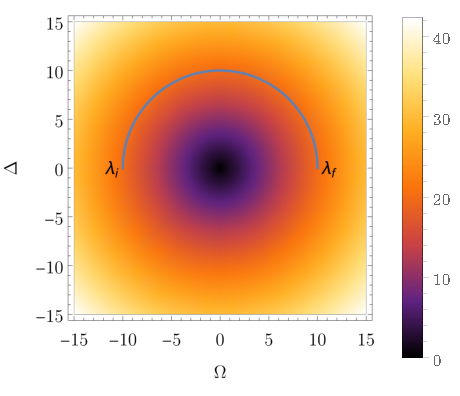
\includegraphics[scale=1.2]{../img/driving.pdf}
    \caption{Driving along the geodesic. DensityPlot shows the difference between Hamiltonian eigenvalues.}
    \label{fig:driving}
\end{figure}

Because the Hamiltonian can be rewritten using Pauli matrices
\begin{equation}
    \H(t) = \Delta(t)\sigma_x+ \Omega(t)\sigma_z
\end{equation}
one can see that changing to moving frame of reference (let's omit the final time dependence $\omega=\omega(T_f)$ for a while and use different colors for different frames) 
\begin{equation}
    \textcolor{purple}{\psi(t)} \eqqcolon \expsm \textcolor{blue}{\tilde\psi(t)}
\end{equation}
reflects rotational symmetry of the problem. This change of reference frame in Schr\"odinger equation is in fact
\begin{equation}
    \begin{split}
        \textcolor{purple}{\H(t)\psi(t)} &= i\textcolor{purple}{\psi'(t)}\\
        \textcolor{purple}{\H(t)} \expsm\textcolor{blue}{\tilde\psi(t)} &= i \expsm \left(-\frac{i\omega\hat\sigma_y}{2}\right)\textcolor{blue}{\tilde\psi(t)}+i\expsm\textcolor{blue}{\tilde\psi'(t)}\\
        \underbrace{\left(\expsp \textcolor{purple}{\H(t)}\expsm- \frac{\omega\hat\sigma_y}{2}\Id\right)}_{\textcolor{blue}{\tilde\H(t)}}\textcolor{blue}{\tilde\psi(t)}&=i\textcolor{blue}{\tilde\psi'(t)}.
    \end{split}
\end{equation}
Therefore we can equivalently solve the Fidelity problem in this new coordinate system.

Hamiltonian in the moving frame is
\begin{equation}
    \textcolor{blue}{\tilde\H}=\textcolor{blue}{\begin{pmatrix}
        -\omega(T_f)/2&-s\\
        -s&\omega(T_f)/2
    \end{pmatrix}},
\end{equation}
which is time independent. The Schr\"odinger equation can now be easily solved using evolution operator
\begin{equation}
    \textcolor{blue}{\UU(t)}=e^{-i\textcolor{blue}{\tilde\H}t}=\textcolor{blue}{\begin{pmatrix}
        \cos{(qt)}-\frac{i\omega}{2q}\sin{(qt)} & -\frac{is}{q}\sin{(qt)}\\
        -\frac{is}{q}\sin{(qt)}&\cos{(qt)}+\frac{i\omega}{2q}\sin{(qt)}
    \end{pmatrix}},
\end{equation}
for $q=\frac{1}{2}\sqrt{4s^2+\omega(T_f)^2}$.

In the original frame we get the evolution of the state $\psi(0)$
\begin{equation}
    \textcolor{purple}{\psi(t)}=\expsm \textcolor{blue}{\UU(t) \tilde\psi(0)} = \underbrace{\expsm \textcolor{blue}{\UU}\expsp}_{\textcolor{purple}{\UU(t)}} \underbrace{\expsm \textcolor{blue}{\tilde\psi(0)}}_{\textcolor{purple}{\psi(0)}}.
\end{equation}
The evolution matrix is then
\begin{equation}
    \textcolor{purple}{\UU(t)}=\textcolor{purple}{\begin{pmatrix}
         \cos (q t)+\frac{i \sin (tqt) (\omega  \cos (t \omega )-2 s \sin (t \omega ))}{2 q} & \frac{i \sin (qt) (2 s \cos (t \omega )+\omega  \sin (t \omega ))}{2 q} \\
         \frac{i \sin (qt) (2 s \cos (t \omega )+\omega  \sin (t \omega ))}{2 q} & \cos (qt)+\frac{i \sin (qt) (2 s \sin (t \omega )-\omega  \cos (t \omega ))}{2 q} \\
        \end{pmatrix}}
\end{equation}
and the evolved wavefunction
\begin{equation}
    \textcolor{purple}{\ket{\psi(t)}}=\textcolor{purple}{\begin{pmatrix}
        \cos (qt)+i \sin (qt) \left(\frac{1}{2} (\omega(T_f) ) \cos (t \omega(T_f) )-s \sin (t \omega(T_f) )\right)\\
        \frac{i \sin (qt)}{q} \left(s \cos (t \omega(T_f) )+\frac{1}{2} (\omega(T_f) ) \sin (t \omega(T_f) )\right).
    \end{pmatrix}}
\end{equation}

Fidelity during the transport is then
\begin{equation}
    F=\left|\textcolor{purple}{\braket{0(t)|\psi(t)}}\right|^2,
\end{equation}
where ground state is
\begin{equation}
    \ket{0(t)}=\mathcal{N}\begin{pmatrix}
        \sec (t \omega (T_f))-\tan (t \omega (T_f))\\
        1
    \end{pmatrix},
\end{equation}
for normalization constant $\mathcal{N}$.